\documentclass[tikz]{standalone}
\usepackage{xcolor}
\definecolor{aksen}{HTML}{F7B538}
\definecolor{latar}{HTML}{171D2B}
\definecolor{bidang1}{HTML}{F7B538}
\definecolor{bidang2}{HTML}{5FA8D3}
\pagecolor{latar}
\color{white}
\begin{document}
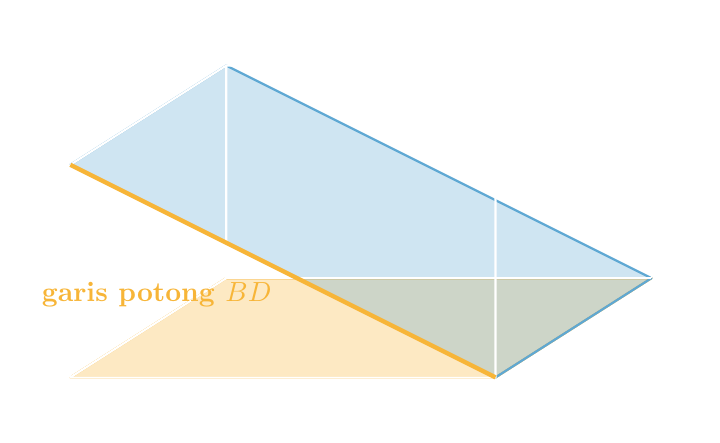
\begin{tikzpicture}[scale=0.9, line join=round]
  \coordinate (A) at (0,0);
  \coordinate (B) at (6,0);
  \coordinate (C) at (6,3);
  \coordinate (D) at (0,3);
  \coordinate (E) at (2.2,1.4);
  \coordinate (F) at (8.2,1.4);
  \coordinate (G) at (8.2,4.4);
  \coordinate (H) at (2.2,4.4);
  % bidang 1: sisi depan ABFE
  \fill[bidang1, opacity=0.30] (A) -- (B) -- (F) -- (E) -- cycle;
  \draw[bidang1, thick] (A) -- (B) -- (F) -- (E) -- cycle;
  % bidang 2: diagonal BDHF
  \fill[bidang2, opacity=0.30] (B) -- (D) -- (H) -- (F) -- cycle;
  \draw[bidang2, thick] (B) -- (D) -- (H) -- (F) -- cycle;
  % rusuk balok (tersembunyi putus-putus)
  \draw[white, dashed] (F) -- (G);
  \draw[white, thick] (A) -- (B) -- (C) -- (G) -- (H) -- (D) -- cycle;
  \draw[white, thick] (A) -- (E) -- (H);
  \draw[white, thick] (E) -- (F);
  % garis potong BD ditebalkan
  \draw[aksen, ultra thick] (B) -- (D) node[midway, below left] {\textbf{garis potong $BD$}};
  % label titik sudut
  \foreach \pt/\pos in {A/below left, B/below right, C/right, D/above left,
                        E/left, F/right, G/right, H/above}
    \node[\pos, white] at (\pt) {$\pt$};
\end{tikzpicture}
\end{document}
